% !TEX root = ../ClassicThesis_DEIB.tex

\chapter{The GRAPE project} \label{chap:grapeProject}

In this chapter, we are going to give a description of the project this thesis work is part of, with particular emphasis on the parts that were specifically addresses in the thesis work. For the description of the project, we make reference to its official proposal.
\ac{GRAPE} is an experimental project of \ac{ECHORD++} and, as hinted in the first part of Chapter \ref{chap:backgroundAndToolsChapter}, it focuses on vineyard farming activities and aims at setting up a robotic manipulation platform able to support lead users to develop a variety of farming applications.
 In effect, the main goal of \ac{GRAPE} is not the complete development of an industrial platform, but, coherently with the research scenario:
\begin{enumerate}
	\item the development of example applications in the pre-mentioned context, exploiting and improving the so-called \textit{key enabling technologies} in robot navigation, perception and manipulation of the project partners; the resulting capabilities are likely to allow to make it easier for small and medium enterprises working in the fields of agricultural robots and, more in general, plant protection.
	\item increase of robot acceptance by farmers and agronomists: since the very last goal of this project is not about the pure research but about the enterprise world, particular attention is given into the realization of a robotic platform that could be accepted by potential end users. For this reason, a constant interaction between the project partners and the potential stakeholders (\textit{i.e.} vinegrowers) is mantained also in development phases.
\end{enumerate}

The example applications have been selected in order to challenge perception and action capabilities, to achieve vineyard monitoring, navigation and manipulation tasks. This decision is taken in the scope of turning traditional farming into precision farming; the realization of such a turn would allow for both the decrease of the chemical load in food and environment, and an improvements of profits and yield for farmers, that would get a return for this investment \parencite{precisionFarming}. The introduction of precision farming tecniques leads indeed to a lot of advantages, for example early detection of plants diseases, or application of pesticides and fungicides with high precision and only when needed.

It's clear that some of these high-precision tasks are still too complex to be automated, and current state-of-the-art in research and technology have been proved to be not yet mature to give rise to a commercial product able to compete with a skilled agricultural agent. The goal of \ac{GRAPE} is creating the enabling technologies to allow agricultural companies to develop vineyard robots to keep filling the gap that exists with respect to traditional methods.

\ac{GRAPE} project specification identify these two application examples:
\begin{itemize}
	\item \textbf{Vineyard monitoring and autonomous navigation}: the developed robotic platform must be able to autonomously navigate the vineyard and localize itself into a map of the environment (downstream a mapping phase), to be able to monitor the state of the vineyard (\textit{e.g.} foliage and grapes inspection). The project implementation focused on a semi-autonomous monitoring, that consider a fully autonomous navigation platoform, with video stream capability that allows human users to observe in person the live data collected by the robot. 
	\item \textbf{Autonomous application of pherormone dispenser applications}: pherormone dispensers are used for \textit{mating disruption} tecniques, to protect grapevines from grape moths, by disrupting the bugs' reproductive cycle making use of synthesized sex pherormones. 
\end{itemize}

\begin{figure}
	\centering
	\subfloat[]{%
		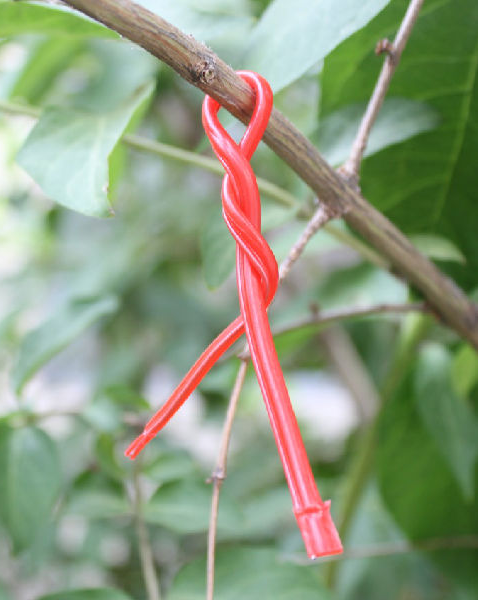
\includegraphics[width=0.3\textwidth]{Images/grape_project/dispenser1.png}
		\label{fig:dispenser1}}
	\qquad
	\subfloat[]{%
		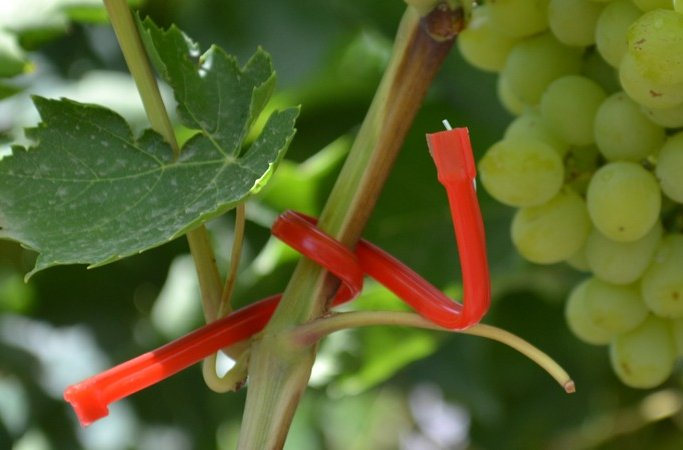
\includegraphics[width=0.3\textwidth]{Images/grape_project/dispenser2.jpg}
		\label{fig:dispenser2}}
	\qquad
	\subfloat[]{%
		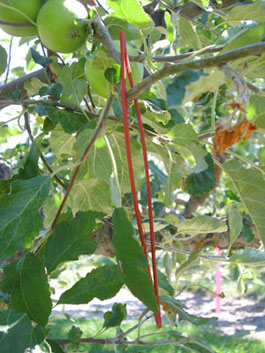
\includegraphics[width=0.12\textwidth]{Images/grape_project/dispenserNostro.jpg}
		\label{fig:dispenserNostro}}
	\caption{\textit{Different shape of pherormone dispensers available on the market. The model used in \ac{GRAPE} is the one depicted in image \ref{fig:dispenserNostro}}}
	\label{fig:dispensers}
\end{figure}


\hrulefill


The GRAPE project chapter SKETCH:
\begin{itemize}
	\item descrizione del progetto e i suoi macro goals: sviluppo piattaforma robotica per applcazi in vigna, aumento dell'accettazione dei robot tra farmers e agronomists. (setting up a robotic manipulation platform able to support lead users to
develop a variety of farming applications.)
	\item mezzi per verification dei macro goal di prima: appication examples della piattaforma di cui sopra  (navigazione autonoma, monitoraggio  della salute della vigna, dispenser dei ferormoni, teleop), e  interfaccia user friendly, collaborazioen con vitirover
	\item modularità necessaria per l'estensiona a una flotta di robots
	\item enti collaborativi (polimi, eurecat, vitirover) con relativi compiti
	\item difficoltà previste: (in order to perform any kind of activity
in a vineyard, the robotic platform has to be able to safely navigate in an outdoor environment characterized by sloping rough terrain), analisi della struttura delle piante in ambiente fortemente non strutturato come la vigna per decisione di punto di deployment, Advanced perception capabilities are essential in manipulation tasks as well, in order to control (e.g.,
by way of visual servoing) the manipulator in a complex, unstructured and dynamic environment.
	\item parti su cui ho lavorato io direttamente (design dell'architettura sw, scan motion, parti del deployment)
	\item related projects [VINEROBOT], [VINBOT], [ROBO-
FARM], [USER-PA], [CROPS], [RHEA] and [SWEPPER] and [FLOURISH])
	\item qualche foto di vigna/dispensers
\end{itemize}

